\subsection{Lecture 25}
\subsubsection{Kalman Filtering}

We first discuss the scalar Kalman Filter.

Consider a system with state $x_n$ and output $y_n$.
\begin{align*}
    x_n &= a x_{n - 1} + v_n \\
    y_n &= cx_n + w_n
\end{align*}
with $|a| < 1$ and $x_0, \{v_n\}_{n =1}^{\infty}, \{w_n\}_{n = 1}^{\infty}$ are zero-mean random variables.
Define $\Var{v_n} = \E{v_n^2} = \sigma_v^2$ and $\Var{w_n} = \E{w_n^2} = \sigma_w^2$.

Our goal is to find $\hat{x}_{n \mid n} = L[x_n \mid y_1, \dots, y_n]$, i.e.
the best linear model of $x$ given observations. The solution is called the Kalman filter.

\begin{theorem}[Scalar Kalman Filter]
    The scalar Kalman Filter has solution given by:

    \begin{enumerate}
        \item Compute $\sigma_{1 \mid 1}^2$ and iterate for $n \geq 2$ using:
        \[ \sigma_{n \mid n - 1}^2 = \E{(x_n - \hat{x}_{n \mid n - 1})^2} = a^2 \sigma_{n - 1 \mid n - 1}^2 + \sigma_v^2 \]
        with
        \[ k_n = \frac{\sigma_{n \mid n - 1}^2}{\sigma_{n \mid n - 1}^2 + \sigma_{w}^2} \]
        where you get $n \mid n$ terms by:
        \[ \sigma_{n \mid n} = \E{(x_n - \hat{x}_{n \mid n})^2} = \sigma_{n \mid n - 1}^2 ( 1 - k_n) \]
        \item Compute $\hat{x}_{1 \mid 1}$, $\sigma_{1 \mid 1}^2$ and iterate for $n \geq 2$ using:
        \[ \hat{x}_{n \mid n} = a \hat{x}_{n - 1 \mid n - 1} + k_n (y_n - a \hat{x}_{n - 1 \mid n - 1}) \]
        where $k_n$'s can be computed offline.
    \end{enumerate}

    \begin{proof*}
        \begin{align*}
            \hat{x}_{n \mid n} &= L[x_n \mid y_1, \dots, y_n] \\
            &= L[x_n \mid y_1, \dots, y_{n - 1}] + L[x_n \mid y_n - L[y_n \mid y_1, \dots, y_{n - 1}]] \\
            &= \hat{x}_{n \mid n - 1} + L[x_n \mid \tilde{y}_n]
        \end{align*}
        Note that everything is 0-mean, so $L[x_n \mid \tilde{y}_n] = k_n \tilde{y}_n$. Then we have,
        \[ \hat{x}_{n \mid n} = \hat{x}_{n \mid n - 1} + k_n \tilde{y}_n \]
        Let's see if we can simplify the former term by utilizing system dynamics.
        \begin{align*}
            \hat{x}_{n \mid n - 1} &= L[x_n \mid y_1, \dots, y_{n - 1}] \\
            &= L[a x_{n - 1} + v_n \mid y_1, \dots, y_{n - 1}] \\
            &= a L[x_{n - 1} \mid y_1, \dots, y_{n - 1}] \\
            &= a \hat{x}_{n - 1 \mid n - 1}
        \end{align*}
        Then, finally,
        \begin{align*}
            \tilde{y}_n &= y_n - L[y_n \mid y_1, \dots, y_{n - 1}] \\
            &= y_n - L[x_n + w_n \mid y_1, \dots, y_{n - 1}] \\
            &= y_n - \hat{x}_{n \mid n - 1}
        \end{align*}
        Thus, we have that:
        \begin{align*}
            \hat{x}_{n \mid n} &= a \hat{x}_{n - 1 \mid n - 1} + k_n(y_n - \hat{x}_{n \mid n - 1}) \\
            &= a \hat{x}_{n - 1 \mid n - 1} + k_n(y_n - \hat{x}_{n - 1 \mid n - 1})
        \end{align*}
        We have the recursion. Now we need to find the constant $k_n$. We can take a geometric approach.
        It is the constant of projection of $x_n$ onto $\tilde{y}_n$. Consider the following diagram:

        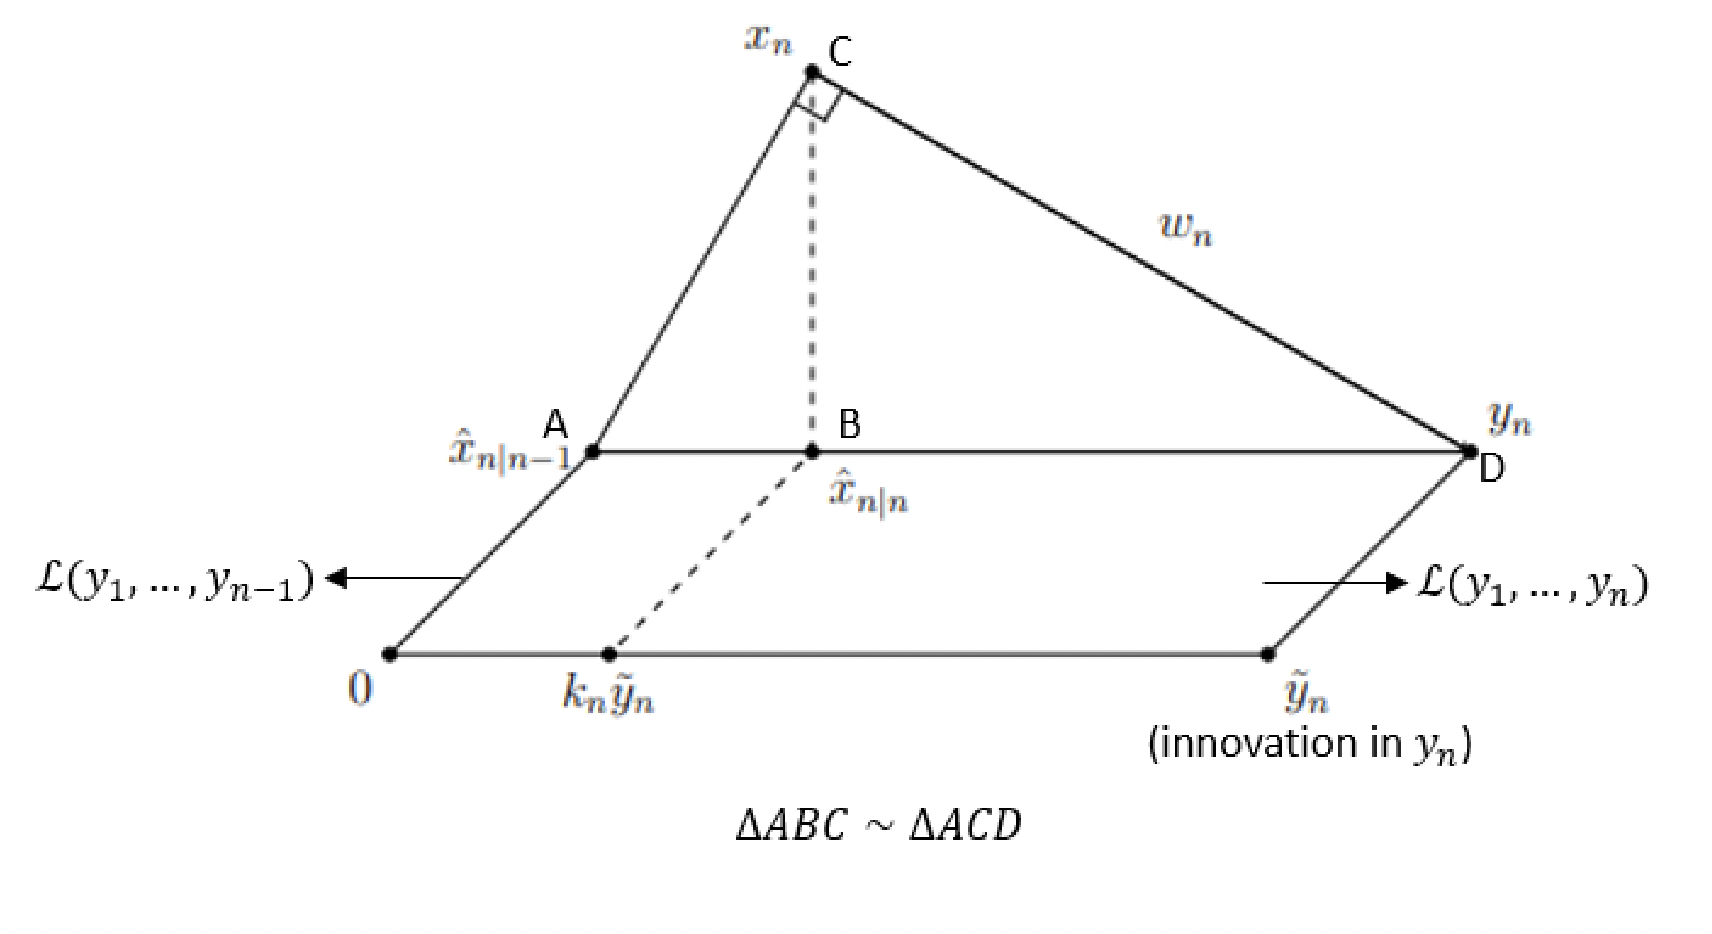
\includegraphics[width=300px]{kalman_proof.png}

        The way we constructed this diagram is as follows.
        \begin{enumerate}
            \item We place the origin 0 and $x_n$. 
            \item We place $\hat{x}_{n \mid n - 1}$ such that $\hat{x}_{n \mid n - 1} \perp (x_n - \hat{x}_{n \mid n - 1})$ (the LLSE is orthogonal to the error).
            \item We place $\tilde{y}_n$ (the error) perpendicular to $L[y_n \mid y_1, \dots, y_{n - 1}] = \hat{x}_{n \mid n - 1}$ (the estimation).
            \item We place $y_n$ such that $y_n = \hat{x}_{n \mid n - 1} + \tilde{y}_n$.
            \item We place $k_n \tilde{y}_n$ as the projection of $x_n$ on $\tilde{y}_n$.
            \item We place $\hat{x}_{n \mid n}$ (the projection onto the plane) such that $\hat{x}_{n \mid n - 1} + k_n \tilde{y}_n$ (this means it lies on the line segment $AB$).
            \item We place $w_n$ such that $x_n + w_n = y_n$.
        \end{enumerate}

        Now, we reason with simple geometry. First, notice that $|AB| = k_n |AD|$. Then, note that $\triangle ABC \sim \triangle ACD$, so
        \begin{align*}
            \frac{|AB|}{|AC|} &= \frac{|AC|}{|AD|} \\
            |AB| &= \frac{|AC|^2}{|AD|} \\
            k_n &= \frac{|AC|^2}{|AD|^2} \\
            k_n &= \frac{|AC|^2}{|AC|^2 + |CD|^2} \\
            k_n &= \frac{\sigma_{n \mid n - 1}^2}{\sigma_{n \mid n - 1}^2 + \sigma_w^2}
        \end{align*}
        where you can interpret the $\sigma_{n \mid n - 1}$ as the variance of the error $x_n - \hat{x}_{n \mid n - 1}$ (i.e. the norm of it squared in Hilbert space jargon).

        Now, we just need equations for $\sigma_{n \mid n - 1}$ updates. To find this, we use another figure.

        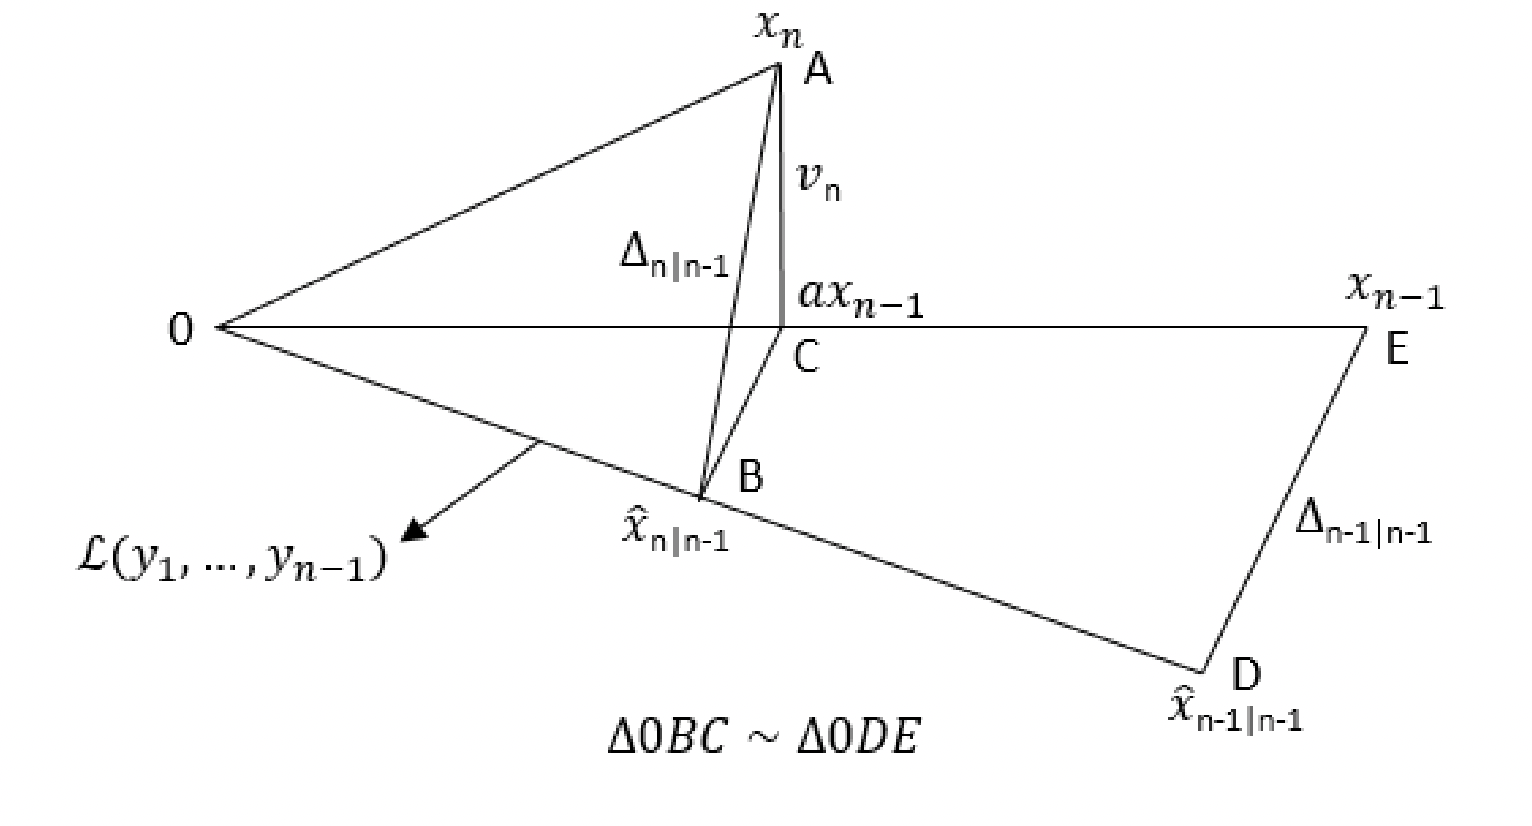
\includegraphics[width=300px]{kalman_proof2.png}

        We constructed this diagram as follows.
        \begin{enumerate}
            \item We place the origin 0 and $x_n$.
            \item We place $\hat{x}_{n \mid n - 1}$ is the projection of $x_n$ on $\mathcal{L}(y_1, \dots, y_{n - 1})$.
            \item We place $\hat{x}_{n - 1 \mid n - 1}$ is the projection of $x_{n - 1}$ on $\mathcal{L}(y_1, \dots, y_{n - 1})$.
            \item We place $x_{n - 1}$, such that $x_n = ax_{n - 1} + v_n$ with $v_n$ orthogonal to $x_{n - 1}$.
        \end{enumerate}

        Now, we want to find the length of the projection error, i.e. $||x_n - \hat{x}_{n \mid n - 1}||^2$ 
        \begin{align*}
            \sigma_{n \mid n - 1}^2 &= || \Delta_{n \mid n - 1} ||^2 \\
            &= |BC|^2 + |AC|^2 \\
            &= |BC|^2 + \sigma_v^2
        \end{align*}
        However, note that $\triangle 0BC \sim \triangle 0DE$. Thus, this means that $|BC| = a ||\Delta_{n - 1 \mid n - 1}|| = a \sigma_{n - 1 \mid n - 1}$,
        so our expression is:
        \[ \sigma_{n \mid n - 1}^2 = a^2 \sigma_{n - 1 \mid n - 1}^2 + \sigma_u^2 \]
        Nice, we have our updates. Now, finally, we need updates for the $n - 1 \mid n - 1$ terms.

        To do this, we return back to our original figure. Note that 
        \begin{align*}
            \sigma_{n \mid n}^2 &= |BC|^2 \\
            &= |AC|^2 - |AB|^2 \\
            &= \sigma_{n \mid n - 1}^2 - k_n^2 |AD|^2 \\
            &= \sigma_{n \mid n - 1}^2 - k_n^2 \frac{|AC|^2}{k_n} \\
            &= \sigma_{n - 1 \mid n - 1}^2 (1 - k_n)
        \end{align*}
        This is the last update. We can update $k_n$ from $\sigma_{n \mid n - 1}^2$, which we can find using $\sigma_{n - 1 \mid n - 1}^2$.
        The recursion is complete.
    \end{proof*}
\end{theorem}

Let us run through an example of doing this.

\begin{example}
    Suppose you know $x_0 = 0$. Then we can feed the recursion.
    \begin{align*}
        x_1 &= v_1 \\
        y_1 &= v_1 + w_1
    \end{align*}
    This means we can find the first estimate by hand.
    \begin{align*}
        \hat{x}_{1 \mid 1} &= L[x_1 \mid y_1] \\
        &= \frac{\Cov{v_1, v_1 + w_1}}{\sigma_v^2 + \sigma_w^2} y_1 \\
        &= \frac{\sigma_v^2}{\sigma_v^2 + \sigma_w^2} y_1 \\
    \end{align*}
    There is one more thing we need by hand.
    \begin{align*}
        \sigma_{1 \mid 1} &= \E{(x_1 - \hat{x}_{1 \mid 1})^2} \\
        &= \E{x_1^2} - \E{\hat{x}_{1 \mid 1}^2} \\
        &= \sigma_v^2 - \frac{\sigma_v^4}{(\sigma_v^2 + \sigma_w^2)^2} \E{y_1^2} \\
        &= \sigma_v^2 - \frac{\sigma_v^4}{\sigma_v^2 + \sigma_w^2}
    \end{align*}
    where the second step comes from Pythagorean Theorem.
    Finally, you can run the recursion for $\{k_n\}$. Once we have these, one can use the $\hat{x}$ recursion to find future predictions based on more data $y$.
\end{example}